\chapter{Introducción}
\label{cap:capitulo1}
\setcounter{page}{1}

La robótica es la ciencia encargada del estudio, diseño, fabricación y utilización de robots, combinando mecánica, electrónica e informática.
La palabra robot viene del término \textit{robota} que, traducido del checoslovaco, sería algo similar a trabajo forzado. Hoy en día se define como un
sistema que utiliza una serie de elementos \textit{hardware} (sensores, actuadores y procesadores) y que está controlado por un \textit{software}
para realizar una tarea concreta.

\section{Evolución histórica de la Robótica}
\label{sec:robotica}

Aunque el término \textit{robot} apareció en los años 20, los autómatas, que son máquinas que imitan la figura y movimientos de un ser animado, existían desde mucho antes.
Varios ejemplos de ellos son el robot de Leonardo, un autómata humanoide diseñado por Leonardo Da Vinci en 1495 que no llegó a ser construido, o el ajedrecista
que Leonardo Torres Quevedo construyó en 1912 que, usando electroimanes por debajo del tablero, era capaz de jugar distintos finales
simples (con pocas piezas en el tablero) contra humanos, consiguiendo siempre la victoria.\\

\begin{figure} [H]
  \begin{center}
      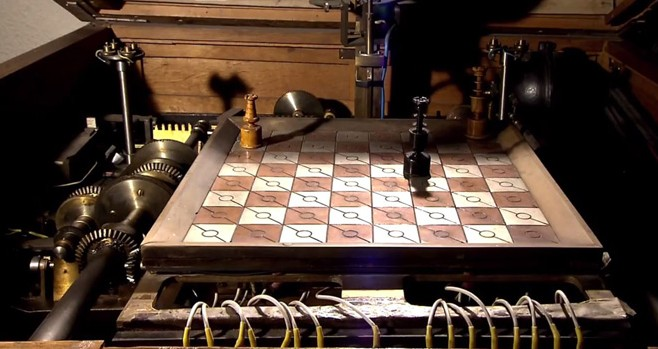
\includegraphics[width=10cm]{figs/c1/ajedrecista.jpg}
  \end{center}
  \caption[El Ajedrecista]{El Ajedrecista. Imagen obtenida de \cite{ajedrecista}}
  \label{fig:ajedrecista}
\end{figure}

En la segunda mitad del siglo XX, con el gran avanze de los ordenadores, se empiezan a ver los primeros robots tal y como se conocen hoy en día.
De esta época debemos destacar al robot industrial que desarrolló la compañía Unimate en 1952, al igual que el robot Shakey, un pequeño robot que apareció
en 1972 capaz de navegar y evitar obstáculos en una habitación cerrada sin interacción humana.

\begin{figure} [H]
  \begin{center}
    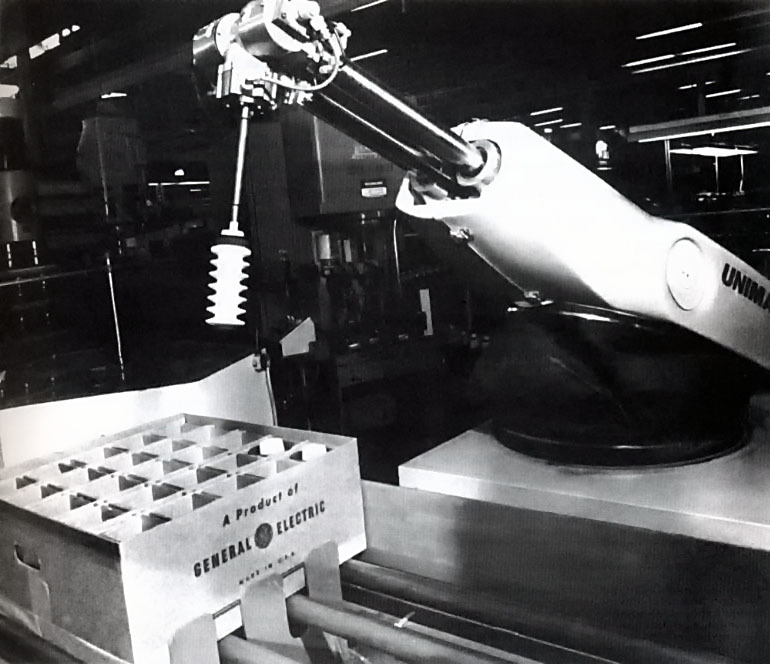
\includegraphics[width=10cm]{figs/c1/unimate.jpg}
    \includegraphics[width=5cm]{figs/c1/shakey.jpg}
  \end{center}
  \caption[Robots Unimate y Shakey]{Robots Unimate y Shakey. Imágenes obtenidas respectivamente de \cite{unimate} y \cite{shakey}}
  \label{fig:unimate_shakey}
\end{figure}

En el 2000, Honda presenta su robot ASIMO (\textit{Advanced Step in Innovative Mobility}), un humanoide que demostró un gran avance en técnicas
complejas como caminar y correr a velocidades de hasta 9km/h.\\

A partir de él surgieron varios robots humanoides con nuevas tecnologías,
como \textit{QRIO} de \textit{Sony} en 2004 siendo capaz de reconocer caras, el pequeño robot \textit{Nao} en 2008 con su habilidad para
interactuar con el ser humano o \textit{Pepper}, un robot con forma humana pero que se desplaza con ruedas que apareció en 2014 y que se usaba sobre todo
como guía o recepcionista, hasta que su desarrollo y producción se abandonó en 2021.

\begin{figure} [H]
  \begin{center}
    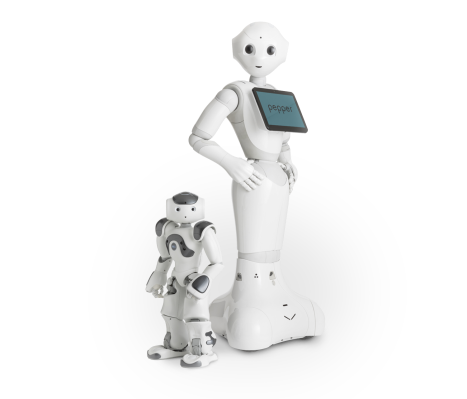
\includegraphics[width=10cm]{figs/c1/nao-pepper.png}
  \end{center}
  \caption[Robots Nao y Pepper]{Robots Nao y Pepper. Imagen obtenida de \cite{nao_pepper}}
  \label{fig:nao_pepper}
\end{figure}

Parejo a estos robots, la NASA estaba desarrollando sus propios robots para mandar a Marte. El \textit{MARS-ROVER}, una plataforma móvil con un brazo mecánico,
sensores de proximidad, láser y cámaras, salió a la luz ya en los años 70. Finalmente su sucesor, el \textit{Sojourner Rover} fue el primero en aterrizar en el
planeta rojo en 1997. En 2004, se lanzaron el \textit{Spirit} y el \textit{Oportunity} con el objetivo de encontrar evidencia de agua, contando con muchos
más sensores e instrumentos científicos que sus predecesores. Las últimas misiones, \textit{Curiosity} y el \textit{Perseverance}, que aterrizaron en
2012 y 2021 respectivamente, tenían el objetivo de buscar indicios de vida en Marte, tanto pasada como presente, a la vez que comprobar si la el desarrollo
de vida humana sería posible.

\begin{figure} [H]
  \begin{center}
    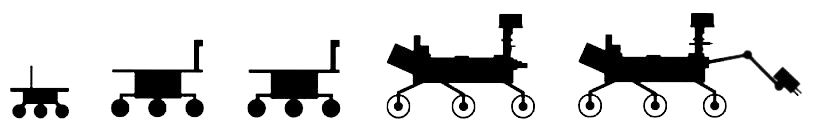
\includegraphics[width=10cm]{figs/c1/rovers.png}
  \end{center}
  \caption[Robots Mars Rovers]{Robots Mars Rovers.}
  \label{fig:rovers_mars}
\end{figure}

Hoy en día, el avance de la robótica ha llegado a una gran variedad de aplicaciones distintas. Entre ellas, podríamos destacar las aplicaciones domésticas
con robots de limpieza como los famosos \textit{Roomba} o iRobot, el sector de la agricultura con vehículos autónomos y monitorizacion de cultivos,
en logística tanto para organizar las mercancías dentro de almacenes como para el reparto, e incluso para conducción autónoma con empresas como Tesla o
Google desarrollando sus propios vehículos que son capaces de conducir grandes distancias sin interacción humana.

\begin{figure} [H]
  \begin{center}
    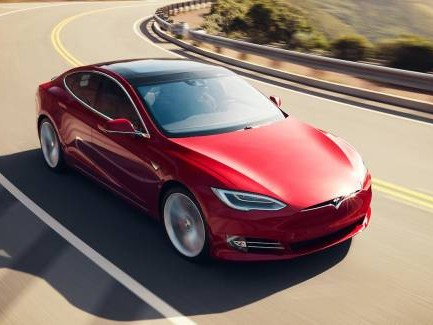
\includegraphics[width=7cm]{figs/c1/tesla-model-s-5_750x.jpg}
    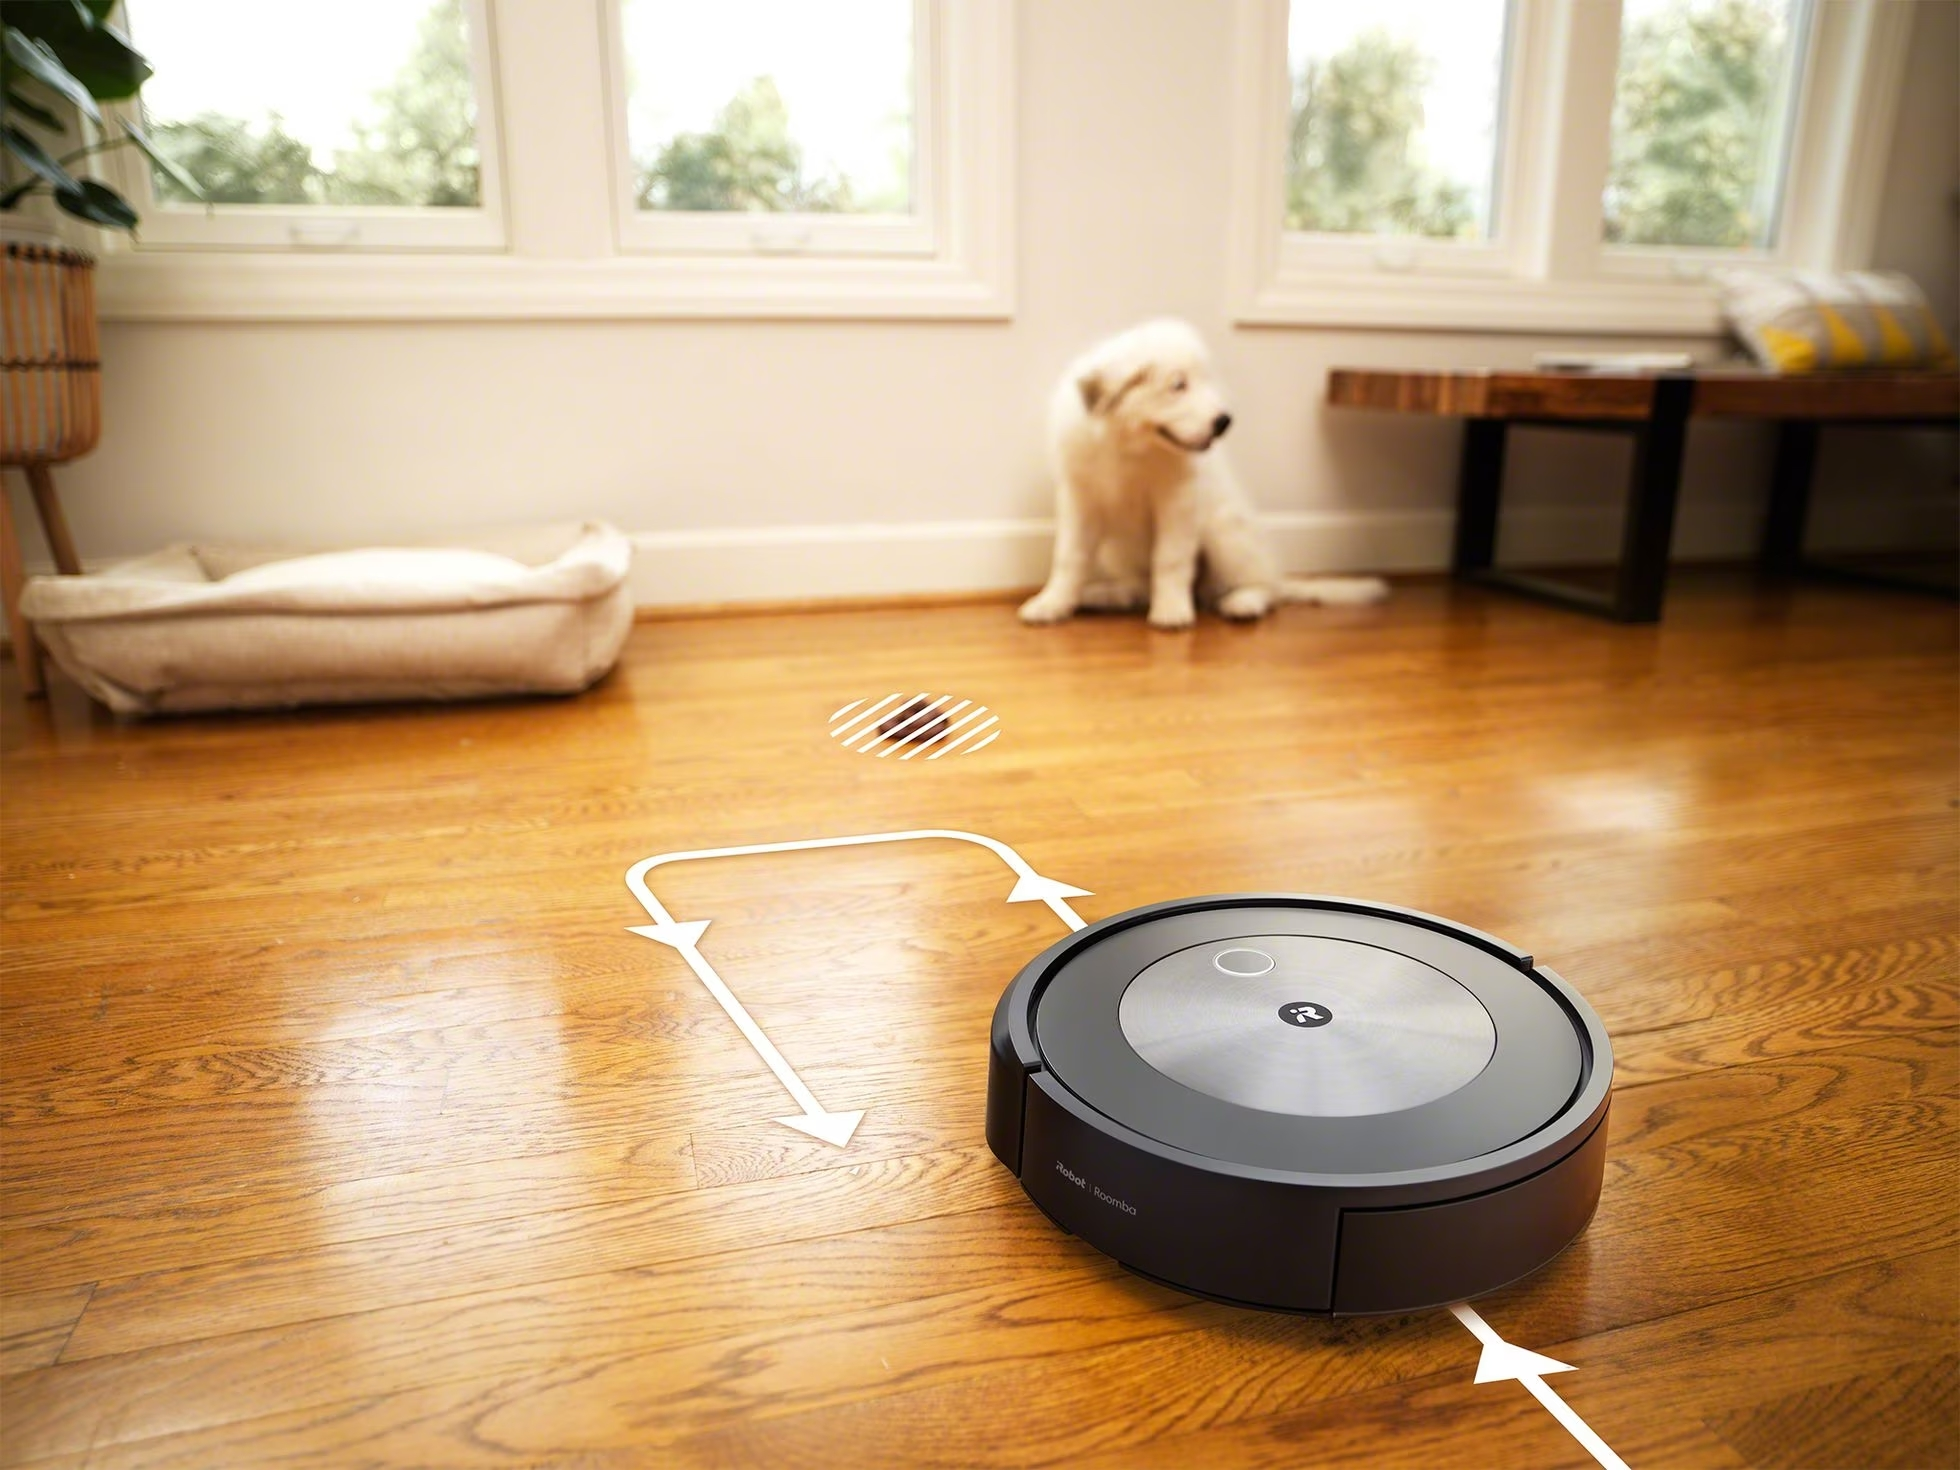
\includegraphics[width=7cm]{figs/c1/roomba.jpg}
    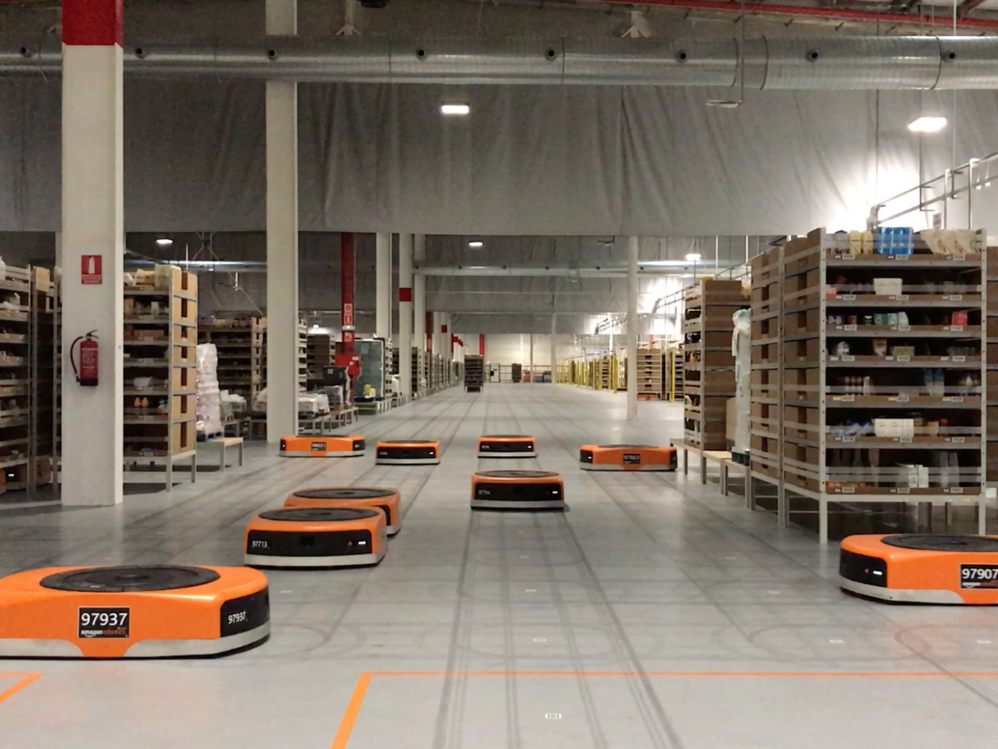
\includegraphics[width=7cm]{figs/c1/almacen.png}
    \includegraphics[width=7cm]{figs/c1/prime.jpg}
  \end{center}
  \caption[Ejemplos aplicaciones actuales robótica]{Ejemplos de aplicaciones actuales de la robótica.}
  \label{fig:rob_varios}
\end{figure}

\subsection{Educación en Robótica}
\label{subsec:urjc}

Actualmente la robótica es un mercado en alza, lo que hace que la cantidad de expertos en el sector sea escasa. 

Los conocimientos de programación es algo que, hasta hace poco, se consideraba algo de nicho y que sólo se enseñaba en algunas universidades, haciendo que
su avance y desarrollo sea lento. Hoy en día se considera algo tan fundamental, que incluso en algunas escuelas primarias se comienzan a desarrollar los
conocimientos en torno a la programación y la robótica con niños de 5 años en las aulas y en talleres.\\

El gran avance en la robótica ha causado una gran demanda de profesionales y, gracias a ello, han surgido grados universitarios como el grado en
Ingeniería de Robótica Software, impartido por la Universidad Rey Juan Carlos en el campus de Fuenlabrada.
Como indica su nombre, este grado está orientado mayoritariamente a la programación, con lenguajes como \textit{python}, \textit{C++} o
\textit{Java}, y abordando temas como inteligencia artificial, ciberseguridad o visión artificial entre otros, todo esto sin dejar de lado
el apartado físico de la robótica, con asignaturas como sensores y actuadores o mecatrónica, donde se enseña a crear robots desde cero.\\

Este grado también da acceso a los estudiantes al laboratorio de
robótica\footnote{\textbf{Laboratorio de robótica}: \url{https://labs.eif.urjc.es/index.php/laboratorios/edificio-laboratorio-iii/laboratorios-laboratorio-l3104/}},
donde podrán programar usando robots reales como el robot Pepper o el TurtleBot2\ref{sec:turtlebot2} usado en este trabajo.

\begin{figure} [H]
  \begin{center}
    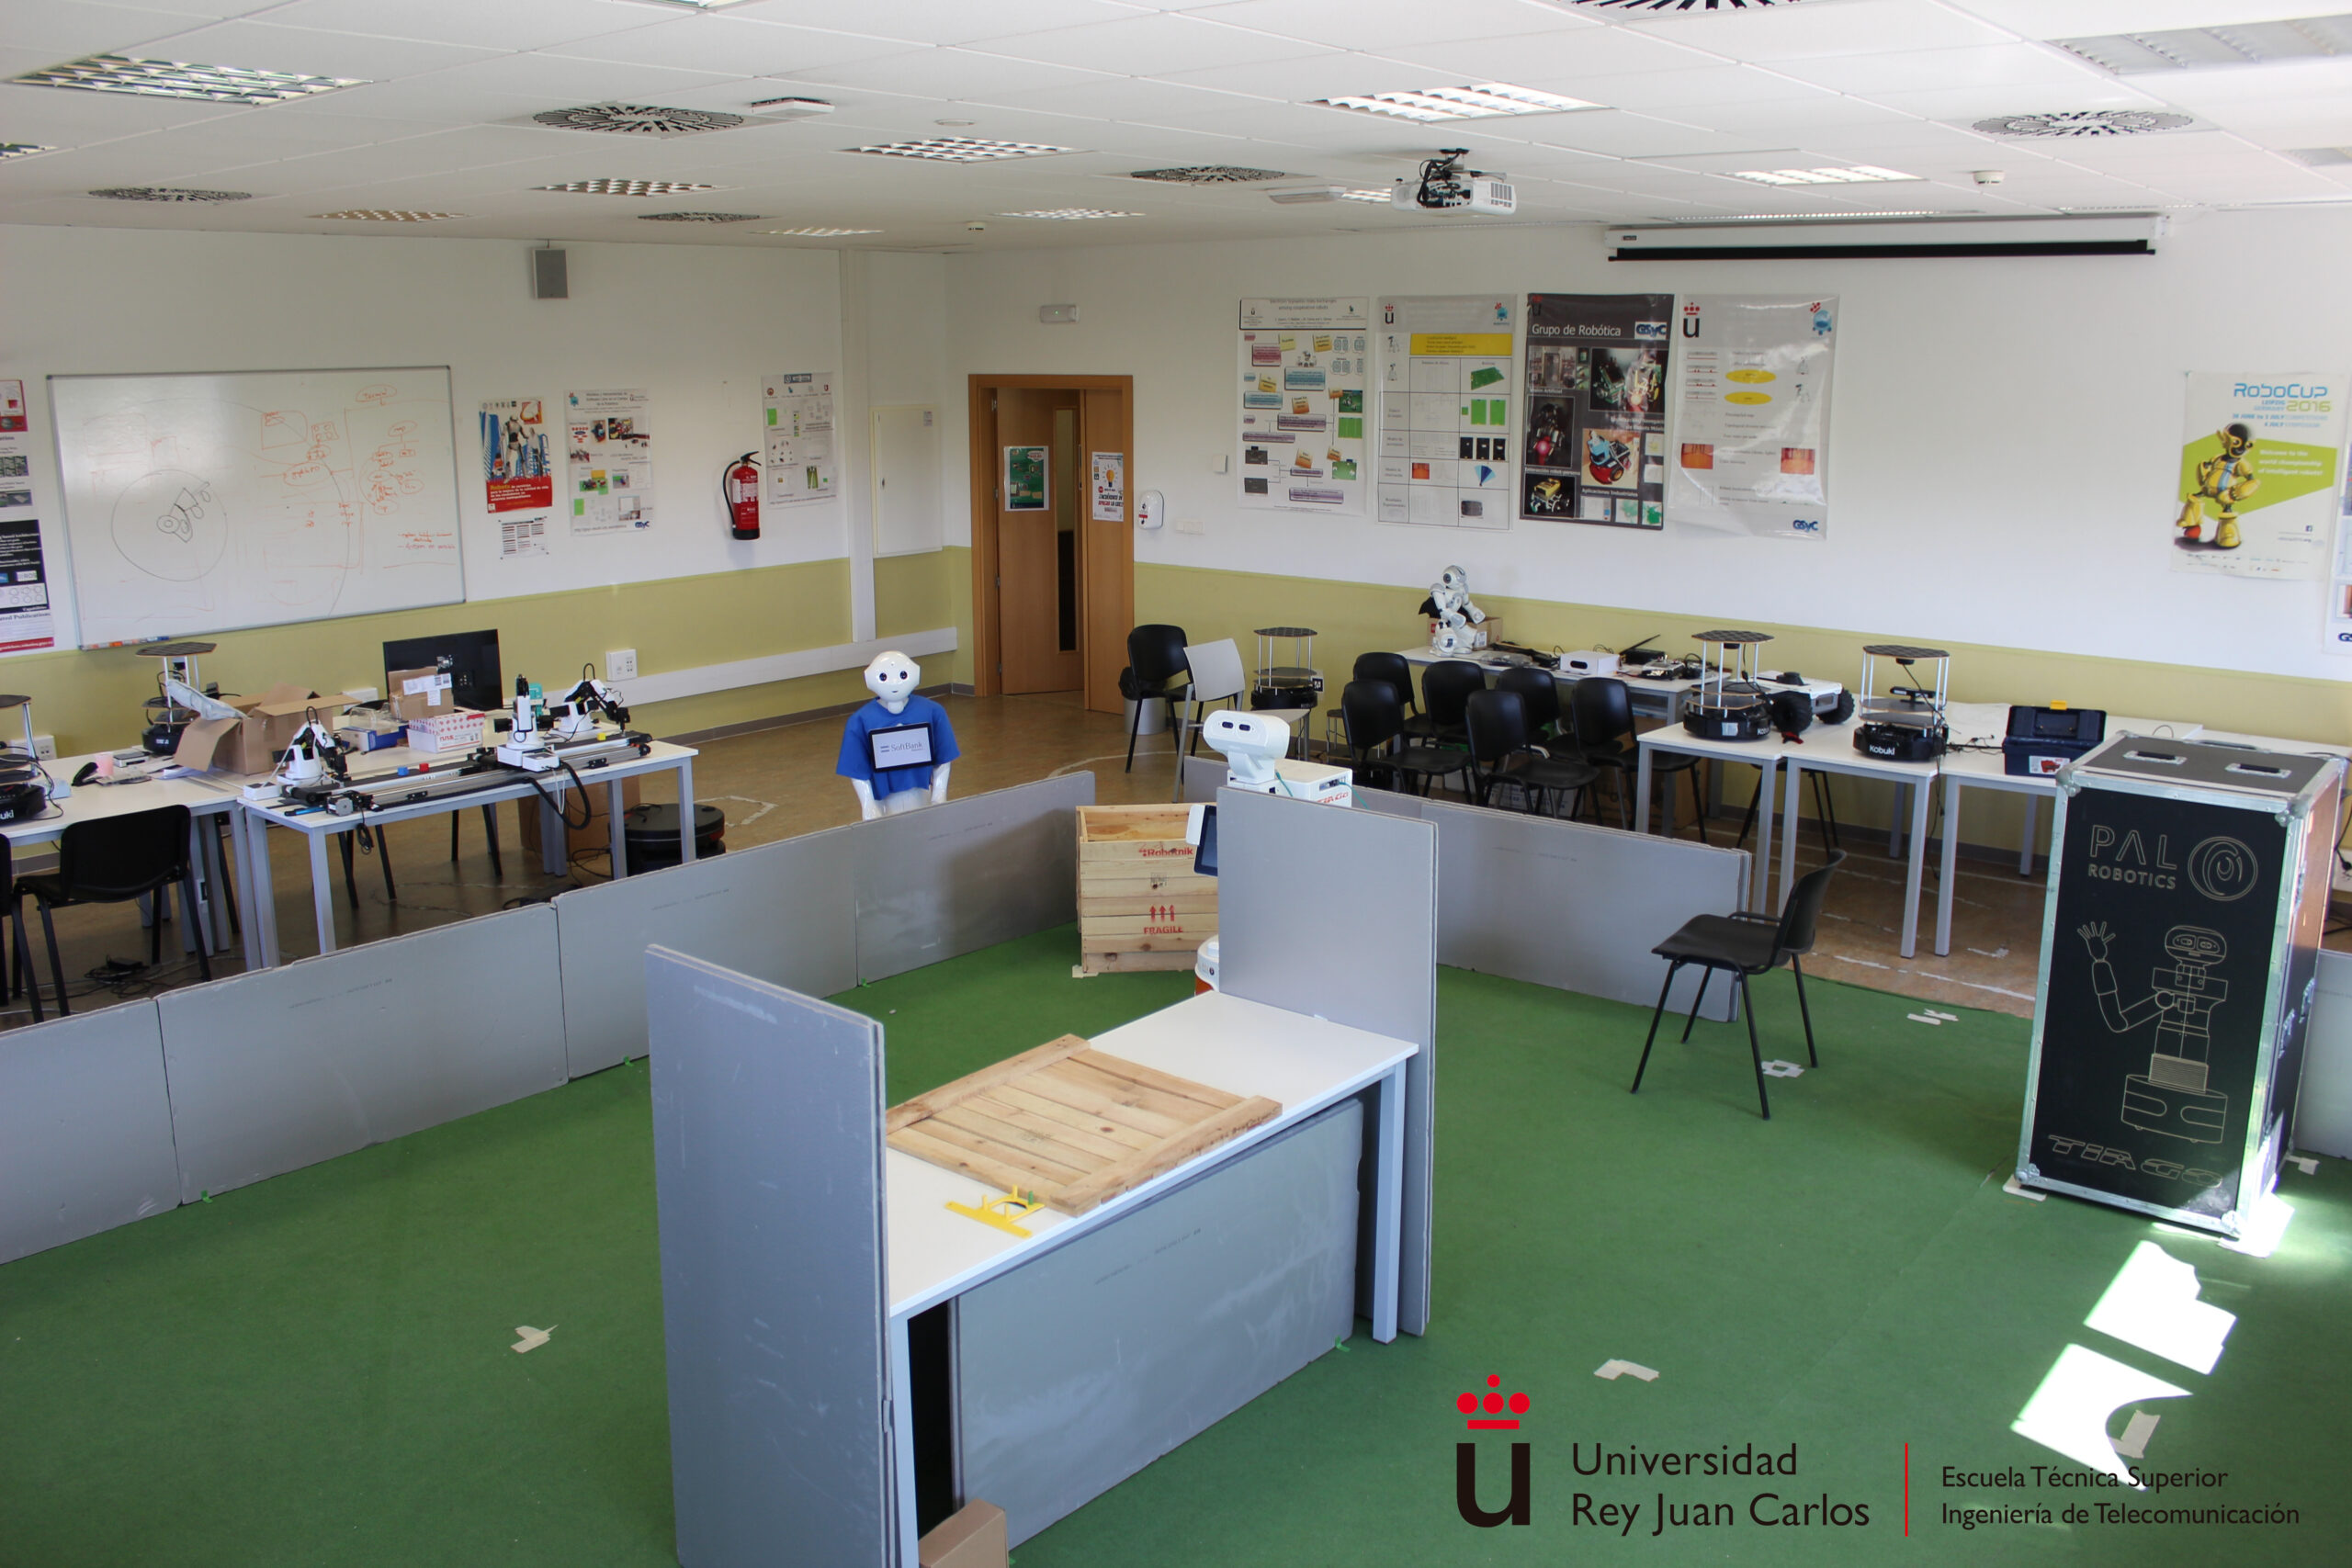
\includegraphics[width=10cm]{figs/c1/rob_lab.jpg}
  \end{center}
  \caption[Laboratorio Robótica]{Laboratorio de Robótica ETSIT.}
  \label{fig:rob_lab}
\end{figure}

\section{Programación de robots}
\label{sec:prog_rob}

El \textit{software} de los robots ha ganado cada vez más importancia a medida que las tareas a realizar se vuelven más complejas.
Gran parte del avance en la robótica se debe a las herramientas que facilitan el desarrollo de este software, como el \textit{middleware} robótico.
El \textit{middleware} más extendido en el mundo de la robótica es ROS (\ref{sec:ros2}). Este nos ofrece una gran variedad de herramientas, desde 
abstracción del hardware, hasta comunicación entre distintas partes del robot. Para usar ROS, lo más común es usar lenguajes de programación como
\textit{python3} o \textit{C++}, aunque ésta no es la única forma de programar robots.

\subsection{Lenguajes de programación visuales}
\label{subsec:vis_prog}

Un lenguaje de programación visual es aquel que permite a los usuarios crear software mediante elementos gráficos y no únicamente mediante texto,
como ocurre con los lenguajes de programación tradicional.

Un gran ejemplo de este tipo de programación es \textit{Scratch}\footnote{\textbf{Scratch}: \url{https://scratch.mit.edu/}}.
Esta plataforma nos permite programar el comportamiento de imágenes conocidas como \textit{sprites} mediante el uso de bloques simples para crear
historias interactivas, animaciones o incluso juegos, permitiendo a los usuarios compartir sus creaciones e investigar cómo lo hacen otros.
Esta plataforma es muy usada en entornos académicos (primaria y secundaria) como introducción a la programación por su simpleza a la hora de entender
conceptos básicos como bucles o condicionales. 

\begin{figure} [H]
  \begin{center}
    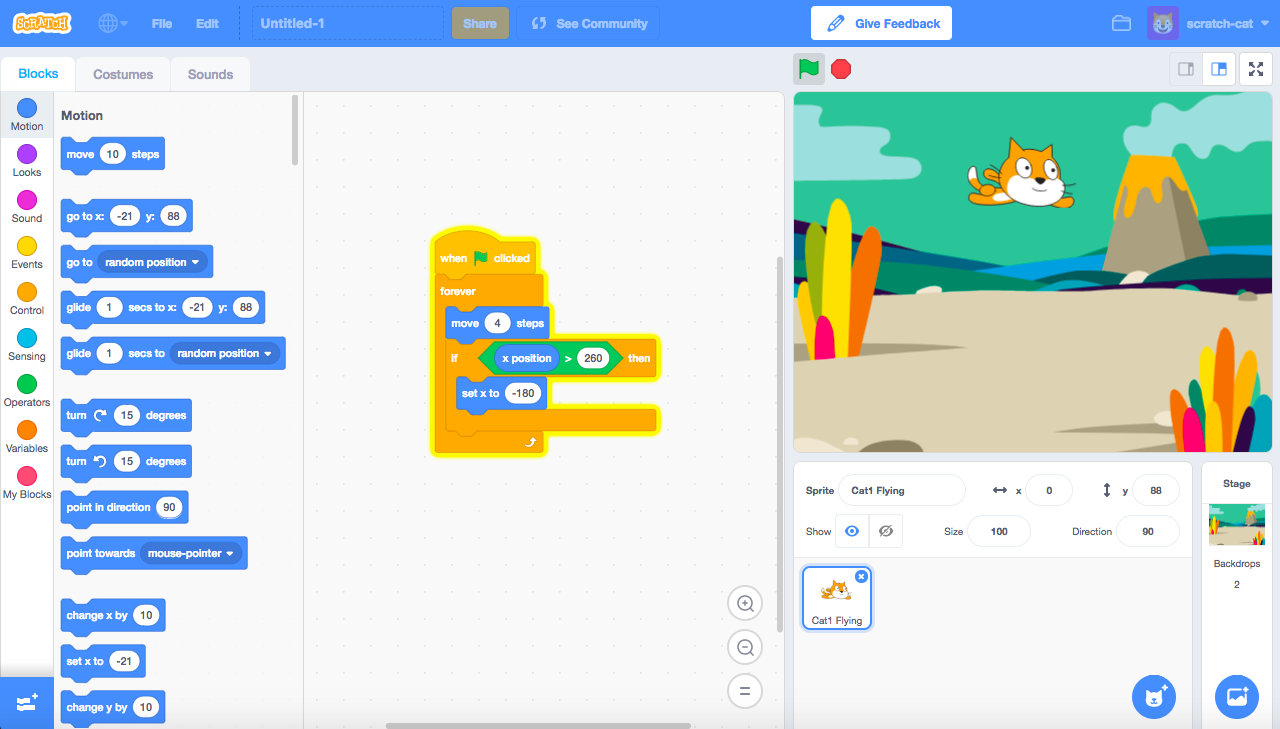
\includegraphics[width=12cm]{figs/c1/scratch.png}
  \end{center}
  \caption[Scratch]{Plataforma Scratch.}
  \label{fig:scratch}
\end{figure}

VisualCircuit, la plataforma en la que se basa este trabajo de fin de grado, también utiliza la programación visual mediante el uso de bloques que se
pueden colocar y unir mediante cables para crear circuitos complejos.
Estos cables envían información entre bloques, desde simples mensajes de texto hasta imágenes o matrices de valores.
La componente visual permite entender el funcionamiento del software sin necesidad de ver cada bloque por dentro.
VisualCircuit nos permite crear aplicaciones robóticas de manera rápida y sencilla sin necesidad de tener grandes conocimientos de programación
o robótica gracias a las librerías de bloques prefabricados que ofrece, destacando bloques de sensores y actuadores (láser, cámara, motores...) o bloques
de edición de imágenes.

\begin{figure} [H]
  \begin{center}
    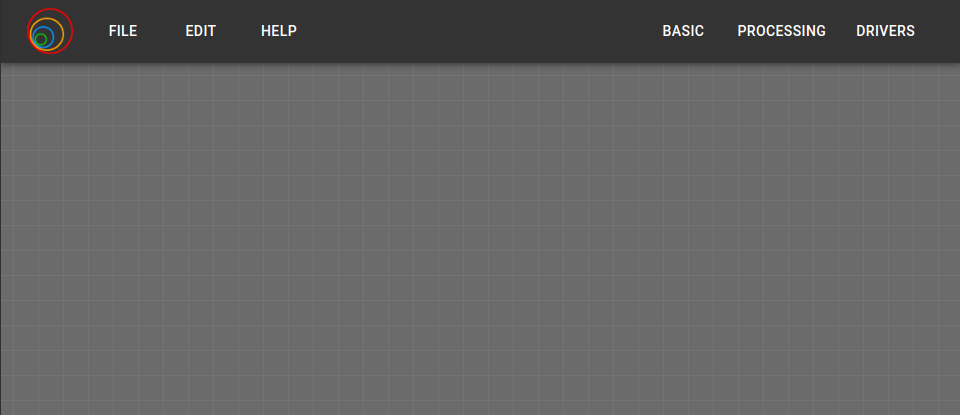
\includegraphics[width=12cm]{figs/c1/empty_VC.png}
  \end{center}
  \caption[Plataforma VisualCircuit]{Plataforma VisualCircuit.}
  \label{fig:VC_plat}
\end{figure}

En el apartado \ref{sec:visualcircuit} se profundizará en el funcionamiento de esta plataforma.